\date{\today}
\newcommand{\doctitle}{Fysik Formelsamling}
\newcommand{\docauthor}{Benjamin Bjørn Ewe}
\newcommand{\docversion}{v0.1.0}

%% using twoside and inner/outer margins for book-like layout
\documentclass[a4paper,12pt,twoside]{article}
\usepackage[
    inner=1.5in,
    outer=0.5in,
    top=1in,
    bottom=1in
    ]
    {geometry} % Smaller margins
%% /using twoside and inner/outer margins for book-like layout


%% Notes
%% This document requires XeLaTeX or LuaLaTeX to compile due to the use of system fonts.
%% Remove the section named "Remove for vanilla LaTeX" if you want to compile with pdfLaTeX.
%%

\documentclass[a4paper,12pt]{article}

%% Custom fonts - Remove for vanilla LaTeX
\usepackage{fontspec}
\setmainfont{RobotoSerif-Regular.ttf}[
    Path = Assets/Fonts/Roboto_Serif/,
    Extension = .ttf,
    BoldFont = RobotoSerif-Bold.ttf,
    ItalicFont = RobotoSerif-Italic.ttf,
    BoldItalicFont = RobotoSerif-BoldItalic.ttf
]
%% /Custom fonts - Remove for vanilla LaTeX
%% Add this if not using XeLaTeX or LuaLaTeX
%\usepackage[utf8]{inputenc}

\usepackage[none]{hyphenat} %% Ensures no hyphenation
\emergencystretch=2em % Alows more empty space between words on lines
\usepackage[final]{microtype} % Improves text appearance - apparently ???

\usepackage{graphics} % for \scalebox
\usepackage{amsmath} % Advanced math typesetting
\usepackage{amssymb} % for math symbols
\usepackage{float} % Improved interface for floating objects
\usepackage[left=1in,right=1in,top=1in,bottom=1in]{geometry} % Smaller margins


\usepackage{tikz} % Advanced drawings
\usetikzlibrary{arrows.meta, angles, quotes}


%% Remove numbering and add symbol before section and subsection titles
\usepackage{titlesec}
\titleformat{\section}
    {\normalfont\Large\bfseries}
    {\thesection \quad}
    {0pt}
    {}
\titleformat{\subsection}
    {\normalfont\large\bfseries}
    {\thesubsection \hspace{0.05em} $-$}
    {0.25em}
    {}
\titleformat{\subsubsection}
    {\normalfont\normalsize\bfseries}
    {}
    {0em}
    {}
\titleformat{\paragraph}
    [runin]
    {\normalfont\normalsize\bfseries\itshape}
    {}
    {0em}
    {}
%% /Remove numbering and add symbol before section and subsection titles

%% Reduce page-break inside sections
\usepackage{needspace}

% discourage page breaks inside paragraphs
\interlinepenalty=10000
\clubpenalty=10000
\widowpenalty=10000
%% /Reduce page-break inside sections.

\setlength{\parindent}{0pt} % No paragraph indentation

%% header and footer
\usepackage{fancyhdr}
\fancyhf{}
\fancyhead[L]{\leftmark}
\fancyhead[R]{\thepage}
\fancyfoot{}
\renewcommand{\sectionmark}[1]{\markboth{#1}{}}
\setlength{\headheight}{14.5pt}
%% /header and footer

% For multiplication table
\usepackage{array}
\usepackage{multirow}
\usepackage{colortbl}
\definecolor{Gray}{gray}{0.85}
\newcolumntype{a}{>{\columncolor{Gray}}c}

\usepackage{tabularray}
\usepackage[x11names]{xcolor}
% /For multiplication table

% For bemærk boxes
\usepackage{xcolor}
\usepackage{tcolorbox}
\tcbuselibrary{breakable}
% /For bemærk boxes

% For pretty tables
\usepackage{booktabs}
% /For pretty tables

% For compact TOC

\usepackage{titletoc}
\titlecontents{section}               % Section
    [0em]                             % Left
    {\vspace*{\baselineskip}}         % Above code
    {\bfseries\thecontentslabel\quad} % Numbered format
    {\bfseries\thecontentslabel}      % Numberless format
    { \textit{S. \thecontentspage}}         % Filler
    []                                % Separator
\titlecontents*{subsection}           % Section
    [0em]                             % Left
    {\space}                          % Above code
    {\thecontentslabel~}              % Numbered format
    {}                                % Numberless format
    {}                                % Filler
    [\hspace{2em}]                    % Separator

\usepackage[hidelinks]{hyperref}
% /For compact TOC
\usepackage{titletoc}
\usepackage{multicol}

\let\sectionSize\small
\let\subsecSize\footnotesize

\renewcommand{\contentsname}{\doctitle} % Change "Contents" title
\titlecontents{section}               % Section
    [0em]                             % Left
    {\sectionSize \vspace{0.4em}}                  % Above code
    {\sectionSize \bfseries \thecontentslabel\quad} % Numbered format
    {\sectionSize \bfseries \thecontentslabel}      % Numberless format
    {\sectionSize \dotfill \thecontentspage}    % Filler
    []                                % Separator
\titlecontents{subsection}            % Section
    [0em]                             % Left
    {}                                % Above code
    {\subsecSize}                          % Numbered format
    {}                                % Numberless format
    {}                                % Filler
    []                                % Separator

\usepackage[hidelinks]{hyperref}

\let\oldtableofcontents\tableofcontents
\renewcommand{\tableofcontents}{
    \newgeometry{left=3cm,right=0cm,top=1cm,bottom=1.5cm}
    \pagestyle{empty} % No headers or footers on TOC page
    \setcounter{tocdepth}{2} % How deep the TOC should go
    \begin{multicols}{2} 
    \oldtableofcontents
    \end{multicols}
    \begin{tikzpicture}[remember picture, overlay]
        \node[anchor=south west, font=\tiny, xshift=3cm, yshift=1cm] at (current page.south west) {\doctitle \space \docversion \space af \docauthor. \space Compiled \today};
    \end{tikzpicture}
    \restoregeometry
}
%% Custom operators
\DeclareMathOperator{\spanop}{Span} % Define \spanop for span operator
\DeclareMathOperator{\nullop}{null}
\DeclareMathOperator{\colsp}{colsp} % Define \colsp for column space
\DeclareMathOperator{\image}{image} % Define \image for image operator
\DeclareMathOperator{\Arg}{Arg} % Define \Arg for argument operator
\DeclareMathOperator{\gm}{gm} % Define \gm for geometric multiplicity
\DeclareMathOperator{\am}{am} % Define \am for algebraic multiplicity
%% /Custom operators

\definecolor{lightmagenta}{rgb}{0.95,0.7,0.95}
\definecolor{lightblue}{rgb}{0.7,0.85,0.95}
\definecolor{lightgreen}{rgb}{0.7,0.95,0.7}

% For bemærk boxes
\newcommand{\bemærk}[1]{%
    \tcbox[
        colframe=lightmagenta,
        boxrule=0.5pt,
        arc=2pt,
        left=6pt,
        right=6pt,
        top=3pt,
        bottom=3pt,
        before upper={\textbf{Bemærk: }},
        on line
    ]
    {#1}%
}

\newcommand{\bemærkBig}[1]{%
    \begin{tcolorbox}[
        colframe=lightmagenta,
        boxrule=0.5pt,
        arc=2pt,
        left=6pt,
        right=6pt,
        top=6pt,
        bottom=6pt,
        before upper={\textbf{Bemærk: }},
        before skip=10pt,    % Space before the box
        after skip=10pt,     % Space after the box
    ]
    #1
    \end{tcolorbox}%
}
% /For bemærk boxes

% For Kilde boxes
\newcommand{\kilde}[1]{%
    \hfill
    \tcbox[
        colframe=lightblue,
        boxrule=0.5pt,
        arc=2pt,
        left=6pt,
        right=6pt,
        top=3pt,
        bottom=3pt,
        on line
    ]
    {\kildeformat#1 \kildeend}%
}

\def\kildeformat#1 #2\kildeend{\textbf{#1} #2}

\newcommand{\kildetag}[1]{%
    \tag*{%
        \tcbox[
            colframe=lightblue,
            boxrule=0.5pt,
            arc=2pt,
            left=2pt,
            right=2pt,
            top=0pt,
            bottom=0pt,
            on line
        ]
        {\formatkildetext{#1}}%
    }%
}

\newcommand{\formatkildetext}[1]{%
    \formatkildetextaux#1 \relax\relax%
}
\def\formatkildetextaux#1 #2\relax{%
    \textbf{#1}%
    \ifx\relax#2\relax\else\ #2\fi%
}
% /For Kilde boxes

% For hidden sections
\newcommand{\hiddensection}[1]{%
    \refstepcounter{section}%
    \sectionmark{#1}%
    \addcontentsline{toc}{section}{\texorpdfstring{\protect\sectionSize #1}{#1}}%
}

\newcommand{\hiddensubsection}[1]{%
    \refstepcounter{subsection}%
    \sectionmark{#1}%
    \addcontentsline{toc}{subsection}{\texorpdfstring{\protect\subsecSize #1}{#1}}%
}
% /For hidden sections

% Change real and imaginary part symbols to 2 letters
\renewcommand{\Re}{\mathfrak{Re}}
\renewcommand{\Im}{\mathfrak{Im}}
% /Change real and imaginary part symbols to 2 letters

% /For Eksempel boxes
\newcommand{\eksempel}[1]{%
    \begin{tcolorbox}[
        colframe=lightgreen,
        colback=white,
        boxrule=1 pt,
        arc=2pt,
        left=6pt,
        right=6pt,
        top=6pt,
        bottom=6pt,
        before upper={\textbf{Eksempel: }},
        before skip=10pt,
        after skip=10pt,
    ]
    #1
    \end{tcolorbox}%
}
% /For Eksempel boxes

% Change ugly empty set symbol
\renewcommand{\emptyset}{\text{Ø}}
% /Change ugly empty set symbol

\newcommand*\cleartoleftpage{%
    \clearpage
    \ifodd\value{page}\hbox{}\newpage\fi
}

\renewcommand{\figurename}{Figur}
\renewcommand{\tablename}{Tabel}

\begin{document}

\pagestyle{empty}
\setcounter{tocdepth}{2}
\tableofcontents

%% Actual start of document
\newpage
\clearpage
\pagestyle{fancy}

% Components

\subsection{Trigonometri}

\subsubsection{Sinus Relationerne}
\begin{minipage}{0.4\textwidth}
    \[
    \frac{a}{\sin(A)} = \frac{b}{\sin(B)} = \frac{c}{\sin(C)}
    \]
\end{minipage}
\hfill
\begin{minipage}{0.4\textwidth}
    \[
    \frac{\sin(A)}{a} = \frac{\sin(B)}{b} = \frac{\sin(C)}{c}
    \]
\end{minipage}

\begin{figure}[H]
    \centering
    \begin{tikzpicture}[scale=1]
        \draw[thick] (0,0) -- (5,0) -- (2.5,4) -- cycle;
        
        % Side labels
        \node at (2.5,-0.3) {c};
        \node at (4.2,2) {b};
        \node at (0.8,2) {a};

        % Point labels
        \node at (-0.2,0) {B};
        \node at (5.2,0) {A};
        \node at (2.5,4.2) {C};

    \end{tikzpicture}
\end{figure}

\subsubsection{Cosinus Relationerne}
\

\begin{minipage}{0.5\textwidth}
    \centering
    \textbf{2 sider og mellemliggende vinkel}
    \[
        a^2 = b^2 + c^2 - 2\cdot b\cdot c\cdot \cos(A)
    \]
    \[
        b^2 = a^2 + c^2 - 2\cdot a\cdot c\cdot \cos(B)
    \]
    \[
        c^2 = a^2 + b^2 - 2\cdot a\cdot b\cdot \cos(C)
    \]
\end{minipage}
\hfill
\begin{minipage}{0.3\textwidth}
    \centering
    \textbf{3 sider}
    \[
        cos(A) = \frac{b^2 + c^2 - a^2}{2\cdot b\cdot c}
    \]
    \[
        cos(B) = \frac{a^2 + c^2 - b^2}{2\cdot a\cdot c}
    \]
    \[
        cos(C) = \frac{a^2 + b^2 - c^2}{2\cdot a\cdot b}
    \]
\end{minipage}

\section{1D mekanik}

$\overline{x}$ betyder gennemsnit af $x$ over et interval.

Det antages at $y$ er positiv opad i formler for tyngdekraft $g$.

Frit fald er uden luftmodstand og med konstant tyngdeacceleration $g$.

\begin{table}[h]
    \begin{minipage}
        {0.65\textwidth}
        \centering
        \renewcommand{\arraystretch}{1.2} % Increase space between rows
        \begin{tabular}{l|l}
            %% Increase space between rows

            \textbf{Begreb} & \textbf{Formel} \\ \hline
            Displacement & $\Delta x = x-x_0$ \\
            Total Displacement & $\Delta x_{total} = \sum \Delta x_i$ \\
            \\
            Average Velocity & $\overline{v} = \frac{\Delta x}{\Delta t} = \frac{v_0 + v}{2}$ \\
            Instantaneous Velocity & $v(t) = \frac{dx}{dt}$ \\
            \\
            Average Speed & $\overline{s} = \frac{\text{Distance}}{\Delta t}$ \\
            Instantaneous Speed & $s = |v(t)|$ \\
            \\
            Average Acceleration & $\overline{a} = \frac{\Delta v}{\Delta t}$ \\
            Instantaneous Acceleration & $a = \frac{dv}{dt}$ \\
            \\
            Position & $x = x_0 + \overline{v} t$ \\
            Velocity & $v = v_0 + \overline{a} t$ \\
        \end{tabular}
    \end{minipage}
    \hfill
    \begin{minipage}
        {0.3\textwidth}
        \centering

        \textbf{Konstant acceleration}
        \begin{align*}
            v &= v_0 + at \\
            x &= x_0 + v_0t + \frac{1}{2}at^2 \\
            v^2 &= v_0^2 + 2a(x-x_0)
        \end{align*}
        \vspace{2em} \\
        \textbf{Frit Fald}
        \begin{align*}
            g &\approx 9.81 \text{ m/s}^2 \\
            v &= v_0 - gt \\
            y &= y_0 + v_0t - \frac{1}{2}gt^2 \\
            v^2 &= v_0^2 - 2g(y-y_0)
        \end{align*}
    \end{minipage}
\end{table}

\textbf{Integration}
\begin{align*}
    v(t) &= \int a(t) dt + v_0 \\
    x(t) &= \int v(t) dt + x_0 
\end{align*}

Fart er absolut hastighed, og hastighed er fart med retning.

$n$ km/h $\approx$ $\frac{n}{3.6}$ m/s

\subsection{Enheds-omregning}
\begin{align*}
    1 \text{ m/s} = 3.6 \text{ km/h} &\iff
    1 \text{ km/h} = \frac{1}{3.6} \text{ m/s} \\
    1 \text{ m/s}^2 = 12.96 \text{ km/h}^2 &\iff
    1 \text{ km/h}^2 = \frac{1}{12.96} \text{ m/s}^2 \\
    1 \text{ radian} = \frac{180}{\pi} \text{ grader} &\iff
    1 \text{ grad} = \frac{\pi}{180} \text{radianer} \\
\end{align*}

\newpage
\section{3D mekanik}

Formlerne for 3D mekanik virker også for 2D mekanik ved at undlade $z$-komponenten.

Når bevægelse i flere dimensioner opdeles i komponenter kan formlerne for hver komponent behandles som 1D mekanik, og de samlede vektorer kan findes ved at kombinere komponenterne.

\subsection{Bevægelse}

\textbf{Position, Hastighed of Acceleration}
\begin{align*}
    \vec r(t) &= x(t) \hat i + y(t) \hat j + z(t) \hat k \\
    \\
    \vec v(t) = \frac{d \vec r(t)}{dt} &= \frac{d x(t)}{dt} \hat i + \frac{d y(t)}{dt} \hat j + \frac{d z(t)}{dt} \hat k \\
    \\
    \vec a(t) = \frac{d \vec v(t)}{dt} &= \frac{d v_x(t)}{dt} \hat i + \frac{d v_y(t)}{dt} \hat j + \frac{d v_z(t)}{dt} \hat k \\
\end{align*}

\textbf{Displacement, og gennemsnitlig hastighed og acceleration}
\begin{align*}
    \Delta \vec r &= \vec r(t_2) - \vec r(t_1) \\
    \\
    \overline{\vec v} &= \frac{\Delta \vec r}{\Delta t} = \frac{\vec r(t_2) - \vec r(t_1)}{t_2 - t_1} \\
    \\
    \overline{\vec a} &= \frac{\Delta \vec v}{\Delta t} = \frac{\vec v(t_2) - \vec v(t_1)}{t_2 - t_1}
\end{align*}

\subsection{Beregning med vinkler og komposanter}

\begin{figure}[th!]
    \centering
    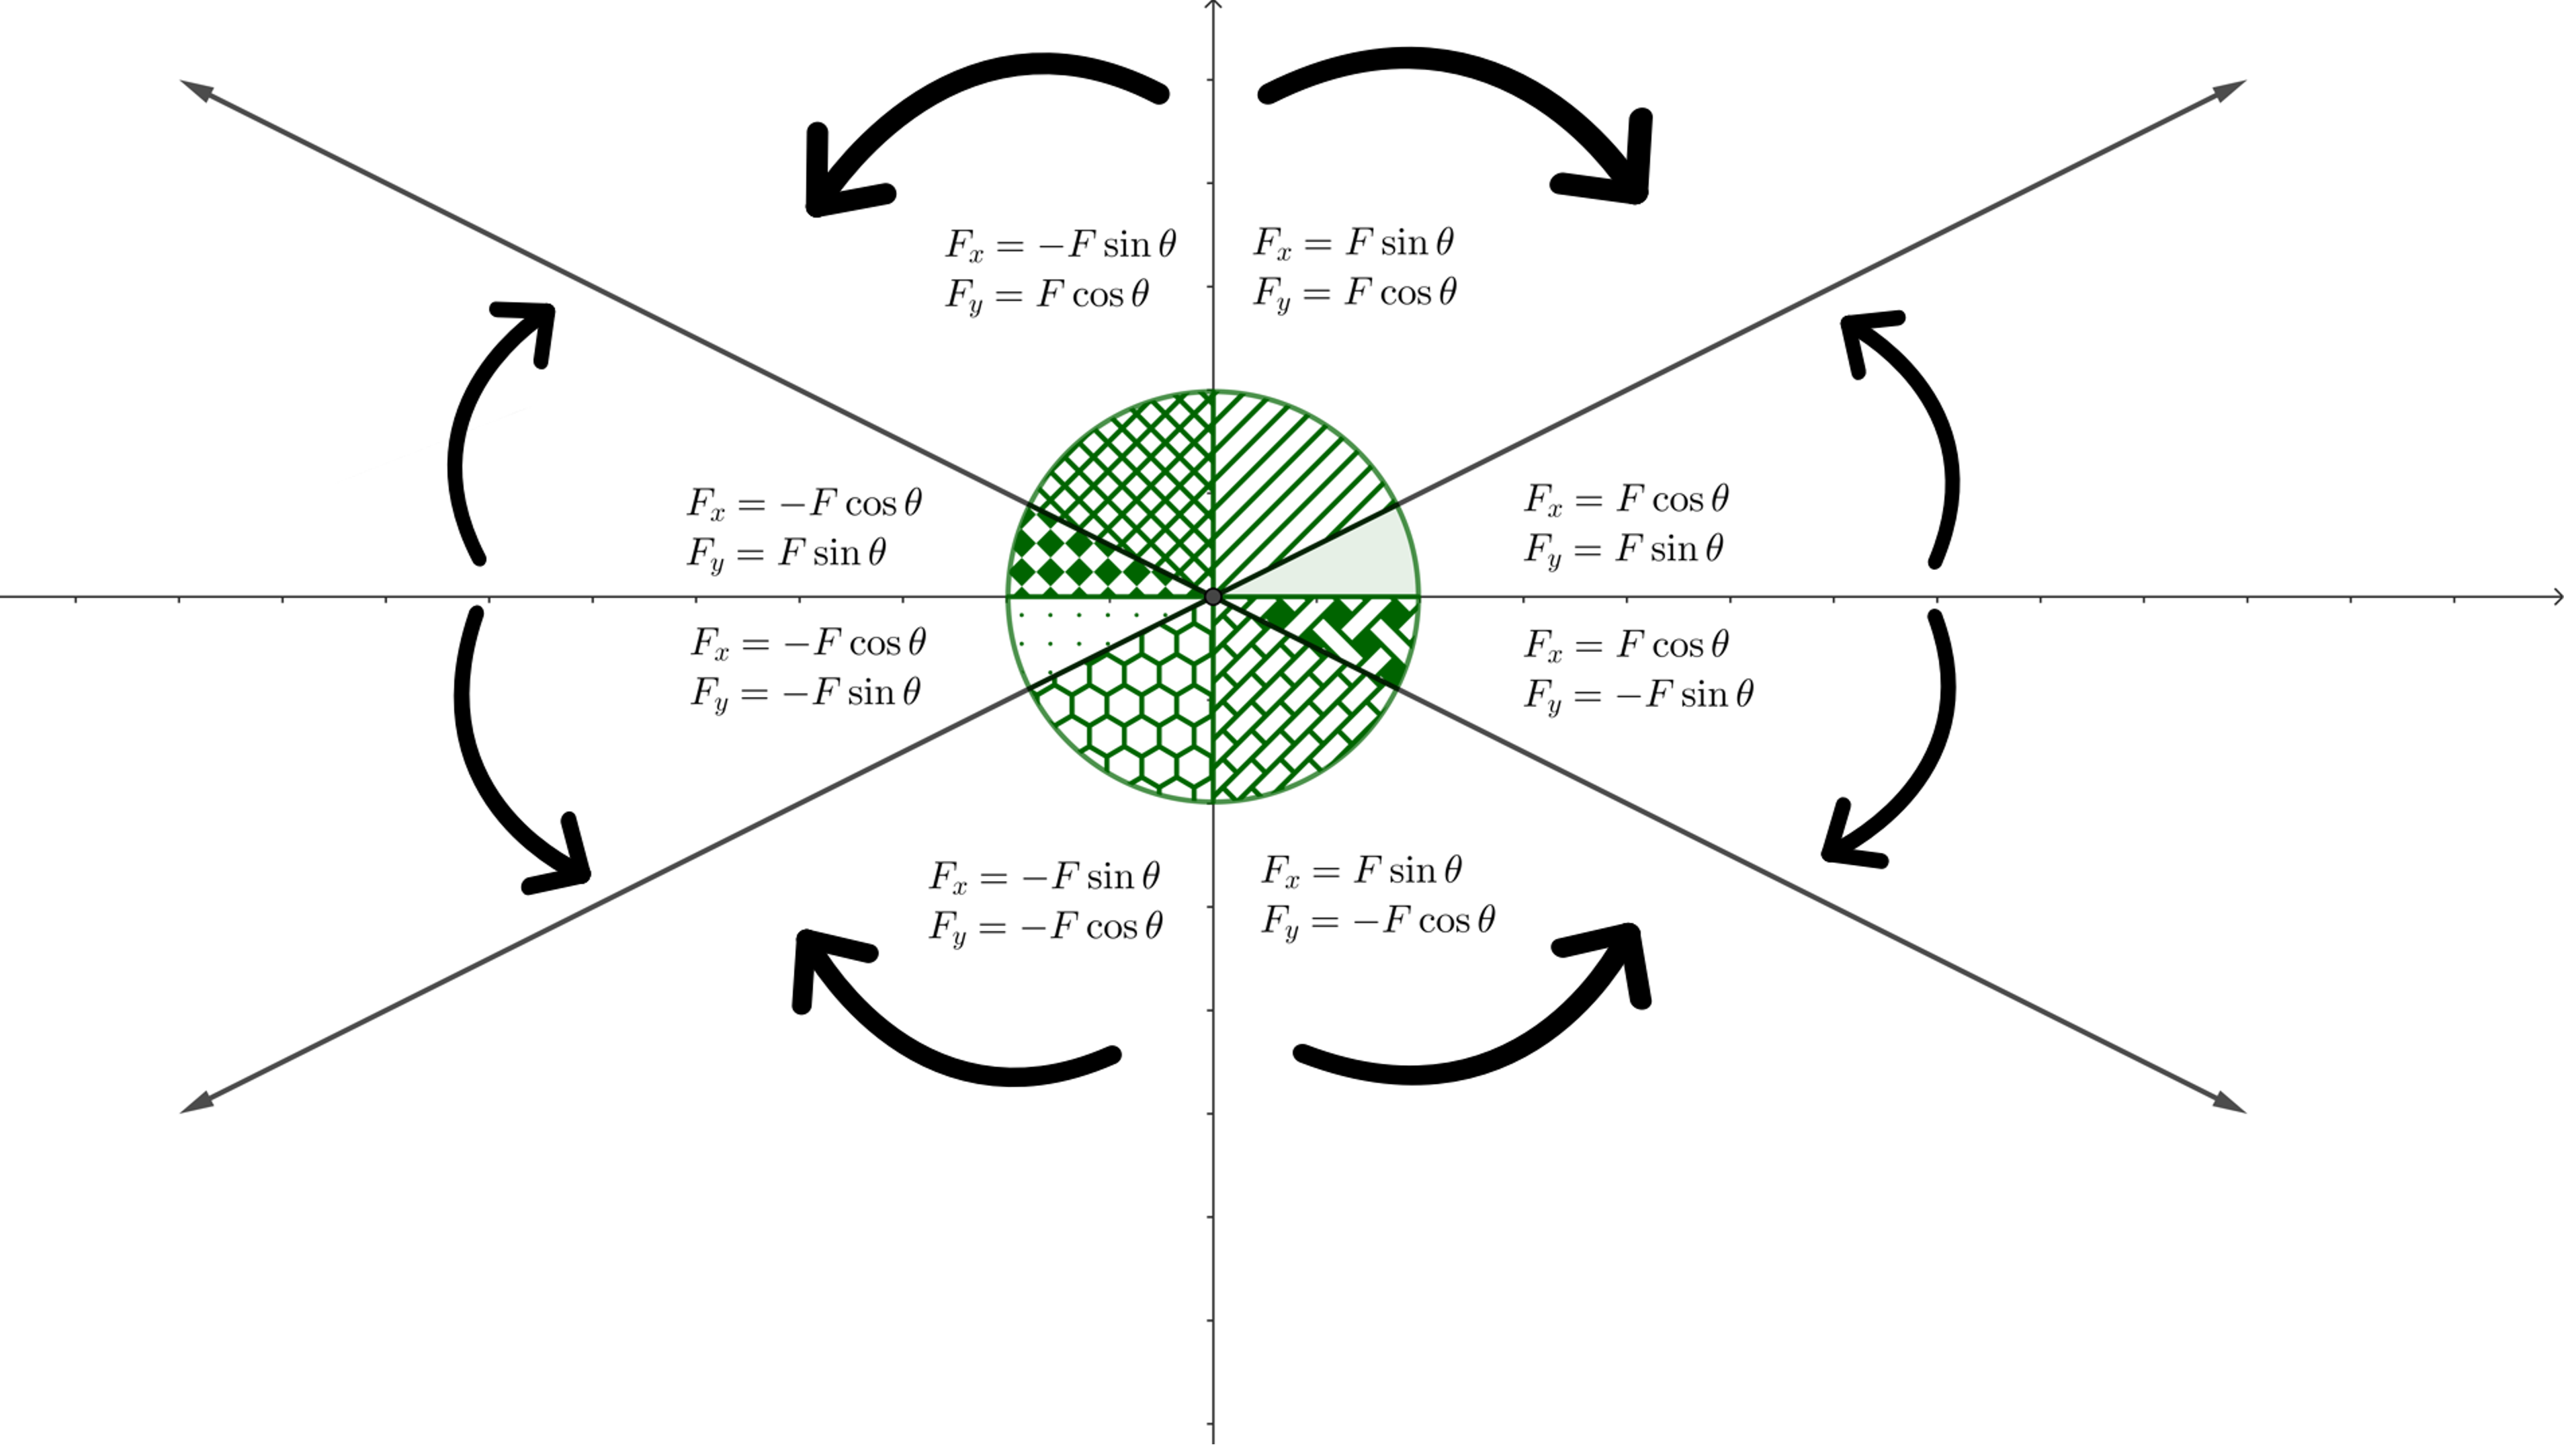
\includegraphics[width=0.8\textwidth]{Assets/Composants/Composants_w_arrows2.png}
    \caption{Komposanter kan findes efter vinkler fra forskellige akser}
    \label{komposanter}
\end{figure}

Givet vektoren $\vec A = A_x \hat i + A_y \hat j$, kan vektorens vinkel $\theta$ og størrelse $A$ findes ved:

\[
    A = \sqrt{A_x^2 + A_y^2} \hspace{6em}
    \theta = \arctan\left(\frac{A_y}{A_x}\right)
\]

Givet vektoren $\vec B$ med størrelse $B$ og vinkel $\phi$ fra den positive $x$-akse, kan vektorens komposanter $B_x$ og $B_y$ findes ved:
\[
    B_x = B \cos(\phi) \hspace{6em}
    B_y = B \sin(\phi)
\]

Generelt: Hvis komposanten man vil finde er \emph{hosliggende} ved vinklen, så bruges cosinus, hvis \emph{modstående}, så bruges sinus.
Se figur \ref{komposanter} for eksempel.

\subsection{Projektil-bevægelse}
2D bevægelse med konstant acceleration i $y$-retningen og 0 acceleration i $x$-retningen.

\subsubsection{Time of Flight}
Gælder kun hvis $y_0 = 0 = y_{\text{final}}$ \hfill $\theta_0$ er vinklen mellem $v_0$ og $x$.

\[
    T_{\text{tof}} = \frac{2 v_0 \sin(\theta_0)}{g}
\]

\bemærk{
    $T_{\text{tof}} \propto v_0$ og $T_{\text{tof}} \propto \frac{1}{g}$
}

\subsubsection{Trajectory}
\[
    y = \tan(\theta_0) \cdot x - \frac{g}{2(v_0 \cos(\theta_0))^2} \cdot x^2
\]

\bemærk{
    Ligningen er på formen $y= ax - bx^2$.
}

\subsubsection{Rækkevidde}
Givet at $x_0 = y_0 = 0$ og $y_{\text{final}} = 0$.
\[
    x = R = \frac{v_0^2 \sin(2\theta)}{g}
\]

\bemærk{
    $R \propto v_0^2$ og $R \propto \frac{1}{g}$.
}

Hvis $\theta_1 + \theta_2 = 90^\circ$ så er $R(\theta_1) = R(\theta_2)$.

\subsubsection{Top-punkt}

\[
    y_{\text{top}} = \frac{(v_0 \sin(\theta_0))^2}{2g}
\]


\subsection{Uniform Cirkulær bevægelse}
Bevægelse i en cirkel med konstant hastighed.

\subsubsection{Centripetal acceleration}

\[
    a_c = \frac{v^2}{r}
\]

Centripetal acceleration peger ind mod centrum af cirklen.

\subsubsection{Centripetal hastighed}
\[
    v = \frac{\text{Circumfrence}}{\text{Period}} = \frac{2\pi r}{T}
\]

\subsubsection{Positions-, hastigheds- og accelerationsvektorer}

\begin{minipage}
    {0.3\textwidth}
    \begin{align*}
        \text{Period of motion: } T &= \frac{2\pi r}{v} \\
        \text{Radius} = r & \\
        \text{Vinkelhastighed: } \omega &= \frac{2\pi}{T} = \frac{v}{r}
    \end{align*}
\end{minipage}
\hfill
\begin{minipage}
    {0.5\textwidth}
    \begin{align*}
        \vec r(t) &= r \cos(\omega t) \hat i + r \sin(\omega t) \hat j \\
        \vec v(t) &= -r\omega \sin(\omega t) \hat i + r\omega \cos(\omega t) \hat j \\
        \vec a(t) &= -r\omega^2 \cos(\omega t) \hat i - r\omega^2 \sin(\omega t) \hat j
    \end{align*}
\end{minipage}

\subsection{Non-uniform Cirkulær bevægelse}
Bevægelse i en cirkel med varierende hastighed, og dermed acceleration ud over den centripetale acceleration.

\subsubsection{Tangentiel acceleration}
\[
    a_T = \frac{d |\vec v|}{dt}
\]
Da $\vec a_T \perp \vec a_c$ gælder 
\begin{align*}
    \vec a_\text{total} &= \vec a_T + \vec a_c \\
    |\vec a_\text{total}| &= \sqrt{a_T^2 + a_c^2}
\end{align*}

\subsection{Relativ bevægelse}
Givet flere vektorer for det samme objekt i forskellige \textit{reference frames}, kan de samles:
\[
    \vec v_{AZ} = \vec v_{AB} + \vec v_{BC} + \vec v_{CD} + \ldots + \vec v_{YZ}
\]
Gælder både for position, hastighed og acceleration.
\include{Components/Physics/Usikkerhed}
\section{Kræfter}

\[
    N = kg \cdot \frac{m}{s^2}
\]

\subsubsection{Newtons Love}
\begin{enumerate}
    \item Et objekt ændrer kun hastighed eller retning hvis det påvirkes af en ekstern kraft.
    \item $F = ma$ (med retning $\vec F = m\vec a$).
    \item For hver handling er der en lige og modsat reaktion.
\end{enumerate}

Den samlede eksterne kraft på et objekt er summen af all eksterne kræfter der påvirker det.

\subsubsection{Vægt}
Vægt defineres $\vec w = m \cdot \vec g$ i vektorform of $w = m \cdot g$ i skalarform.

\subsubsection{Normalkraft}
Normalkraften virker vinkelret på en overflade. 
\[
    N = mg \cos(\theta) \hspace{6em} \text{(På en horisontal overflade er } N = mg\text{)}
\]

\subsubsection{Snor-kraft}
Snor-kraften er kraften langs snoren. 
\[
    T = m \cdot a \sin(\theta) \hspace{6em} \text{(Ved 90° vil } T = mg\text{)}
\]

En vægt midt på en horisontal snor giver snor-kraften:
\[
    T = \frac{mg}{2 \sin(\theta)}
\]
Hvor $\theta$ er vinklen mellem snoren og den horisontale linje.

\subsubsection{Fjeder-kræft}
Fjeder-kræften modarbejder forlængelsen og kompression.
\[
    F = k \cdot x \kildetag{Hookes lov}
\]
Hvor $k$ er fjederkonstanten og $x$ er fjederens forlængelse eller kompression.

\subsection{Friktion}
Statisk friktion $f_s$ er friktionen før et objekt bevæger sig, kinetisk friktion $f_k$ er friktionen mens det bevæger sig.
\[
    f_s \le \mu_s N \hspace{6em} f_k = \mu_k N
\]
Hvor $\mu_s$ og $\mu_k$ er de statiske og kinetiske friktionskoefficienter, og $N$ er normalkraften.

\[
    \mu_k \le \mu_s
\]


\subsubsection{Friktion på hældninger}
Friktionskraften på en hældning er:
\[
    f = \mu_k \cdot m \cdot g \cdot \cos(\theta)
\]
Og accelerationen på en hældning er:
\[
    a = g \cdot (\sin(\theta) - \mu_k \cdot \cos(\theta))
\]
Hvis et objekt bevæger sig ned ad en hældning med konstant fart, er friktions-koeffienten:
\[
    \mu_k = \tan(\theta)
\]

\subsection{Centripetal kraft}
Centripetal kraften er den kraft der kræves for at holde et objekt i en cirkulær bane, og peger mod centrum af cirklen.
\[
    F_c = m \cdot a_c = m \cdot r \cdot \omega^2 = m \frac{v^2}{r}
\]

\subsection{Krængede kurver}
Bevægelse langs en krænget kurve giver en centripetal kraft der peger mod indersiden af kurven, uden at bruge friktion til at opnå det.

\subsubsection{Perfekt Krængning}

En perfekt krængning er en krænget kurve hvor ingen friktion er nødvendig for at holde objektet på banen. Sammenhængen mellem krængningsvinklen $\theta$ og hastigheden $v$ er:
\[
    \tan(\theta) = \frac{v^2}{r \cdot g}
\]

\subsection{Luftmodstand}
Luftmodstand virker mod bevægelsesretningen af objekter der bevæger sig gennem væsker.
\[
    F_D = \frac{1}{2} \cdot \rho \cdot v^2 \cdot C \cdot A
\]
Hvor $\rho =$ væskens densitet, $v =$ hastighed, $C =$ luftmodstands-koefficienten, og $A =$ tværsnitsarealet af objektet.

\subsubsection{Terminal-hastighed}
Terminal-hastigheden er hastigheden påkrævet for $F_D = mg$:
\[
    v_t = \sqrt{\frac{2mg}{\rho C A}}
\]

\subsubsection{Stoke's Lov}
Stoke's lov beskriver luftmodstand for små objekter i en væske:
\[
    F_D = 6 \pi \eta r v
\]
Hvor $\eta =$ væskens viskositet, $r =$ radius af objektet, og $v =$ hastighed.




\end{document}